% !TeX spellcheck = da_DK
\subsection{Software}
\subsubsection{Teori og design}
Efter konverteringen af det analoge signal til digitalt i ADC’en indsendes data til en computer. Jævnfør afsnit \ref{subsec:software}, side \pageref{subsec:software} skal patienternes data behandles i form af grafisk visualisering af deres hældningsresultater, samt gemmes til senere brug og analyse. For at imødekomme disse krav, bruges en computer med software programmerne; Scopelogger og Matlab, hvor Scopelogger anvendes til at optage det  digitale signal fra NIDAQ'en og Matlab benyttes til at behandle opsamlede data. Til behandling og lagring af data udarbejdes en manual for at gøre pogrammets design brugervenligt for det fagkyndige personale, som skal bruge disse data til analyse af patienternes udvikling ift. balancefunktionen. For at programmet skal kunne fungere med en switch knap, jævnfør afsnit \ref{formål_anvendelse}, side \pageref{formål_anvendelse} skal patienternes øvelsesresultater gemmes alt efter pågældende udførte øvelse hhv. 'anatomisk\_data' og 'SRT\_dato'. 
Det fagkyndige personale skal åbne scriptet 'Patient\_Oevelse' i Matlab for at kunne køre computerprogrammet, der skal behandle apopleksipatienternes data fra Scopelogger. Indsamlede data navngives alt efter den pågældende øvelse, der er udført og hentes ind i Matlab. Af nedestående flowdiagram \ref{Flow_manual} fremgår computerprogrammets manual.

\begin{figure}[H] 
	\centering 
	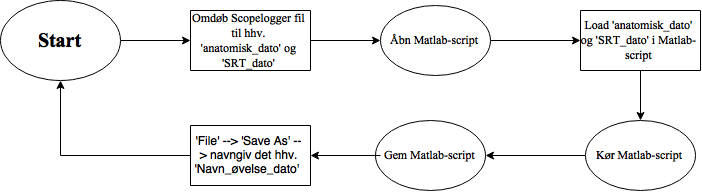
\includegraphics[scale=0.5]{figures/cProblemloesning/Flow_manual.PNG}
	\caption{af flowdiagrammet fremgår computerprogrammets manual, der omhandler hvorledes det fagkyndige skal behandle og gemme apopleksiatienterne øvelsesresultater}
	\label{Flow_manual}
\end{figure} 

Når patientens pågældende øvelse er loadet i Matlab-scriptet ændres grafens titel ift. patientens navn og dato på hvornår øvelsen er udført. Efter Matlab-scriptet er kørt vil der fremkomme en graf af patienternes hældning, hvor tærskelværdierne vil være markeret med horisontale linjer i hhv. gul, grøn, rød og sort. Det fagkyndige personale kan derfor se, hvor hyppigt patienterne har bevæget sig ud i det enkelte risikozoner. Derudover kan det fagkyndige personale ændre på grafens tidsaksen, så der er mulighed for at udvælge data i en bestemt tidsperiode, da selvtrænings sessionen kan have forskellig varighed afhængig af den enkelte patient. På denne måde kan det fagkyndige personale udvælge og undersøge data i en specifik tidsperiode, hvis dette har interesse for analysen af patienternes øvelsesresultater.  

\subsubsection{Implementering og test}
For at teste computerprogrammet foretages en testmåling af hele systemet og efter konverteringen i ADC'en anvendes ovenstående manual til at visualisere en graf, samt gemme data. 

TEST AF SOFTWARE IND HER. TJEK AT VI TESTER FOR KRAVSPECIFIKATIONER


Blokken indeholdende softwaren implementeres i systemet for at kunne behandle og gemme patienternes øvelsesresultater. Denne del af systemet er brugerfladen for det fagkyndige personale og skal derfor kunne fremvise information omkring patienternes balance i form af grafer eller lignende. Det fagkyndige personale skal vha. af softwaren kunne følge med i patienternes udvikling ift. balancen. \\
\textbf{Krav:}
\begin{itemize}
	\item Skal kunne fremvise data med information om patientens hældning i de enkelte øvelser, herunder hvor ofte patienten har bevæget sig ud i risikozonerne. 
	\item Skal kunne gemme data med information om patientens hældning.
	%\item Skal være brugervenligt for det fagkyndige personale, dvs. designet af programmet skal være enkelt. 
\end{itemize}
\textbf{Tolerance:}
\begin{itemize}
	\item Der accepteres ingen afvigelse ift. software. 
\end{itemize}

%Vi kunne for at gøre programmet mere brugervenligt udarbejde en manual til systemet. Derudover kunne det være fordelagtigt at det fagkyndige personalet at have mulighed for at ændre akserne, og her tænkes specielt tidsaksen. Dette tænkes da systemet skal kunne optage selvtræning og da det ikke forventes at patienten tænder og slukker systemet efter hver enkelt øvelse. Dette vil både være svært at huske for patientgruppe (gamle og måske med kognitive komplikationer) og så ville de måske glemme at slå den til igen. Derfor tænkes det at de lader systemet optage signaler under hele selvtrænings sessionen. Det vil midlertidigt blive til utrolig meget data, hvor en stor del af dataen vil være pauser for patienten og derved ubrugelig data for det fagkyndige personale. Det ville derfor være smart at hvis de forholdsvis nemt kunne udvælge perioder i dataen, de gerne vil undersøge nærmere. 
%Derudover skal vi også have gjort patienten og det fagkyndige personale opmærksomme på hvilken øvelse der foretages!
%Det kunne måske være en ide, at vi i grafen kunne ligge tærskelværdierne ind som en form for linjer, så det blev nemmere at aflæse grafen
%Skal vi have en løbende visning af signalet i en graf eller er det bare til sidst! 

%Vores program skal altså kunne:
%  -Optage signalet
% - Behandle signalet således, alt efter sværhedsgrad 
%  - Plotte signalet
% - Gem data'en 
